\documentclass[14pt]{extbook}
\usepackage{multicol, enumerate, enumitem, hyperref, color, soul, setspace, parskip, fancyhdr} %General Packages
\usepackage{amssymb, amsthm, amsmath, latexsym, units, mathtools} %Math Packages
\everymath{\displaystyle} %All math in Display Style
% Packages with additional options
\usepackage[headsep=0.5cm,headheight=12pt, left=1 in,right= 1 in,top= 1 in,bottom= 1 in]{geometry}
\usepackage[usenames,dvipsnames]{xcolor}
\usepackage{dashrule}  % Package to use the command below to create lines between items
\newcommand{\litem}[1]{\item#1\hspace*{-1cm}\rule{\textwidth}{0.4pt}}
\pagestyle{fancy}
\lhead{Progress Quiz 9}
\chead{}
\rhead{Version A}
\lfoot{9541-5764}
\cfoot{}
\rfoot{Summer C 2021}
\begin{document}

\begin{enumerate}
\litem{
Determine the horizontal and/or oblique asymptotes in the rational function below.\[ f(x) = \frac{6x^{3} -43 x^{2} +86 x -40}{3x^{2} -11 x + 6} \]\begin{enumerate}[label=\Alph*.]
\item \( \text{Horizontal Asymptote of } y = 2.0  \)
\item \( \text{Horizontal Asymptote of } y = 3.0 \text{ and Oblique Asymptote of } y = 2x -7 \)
\item \( \text{Horizontal Asymptote of } y = 2.0 \text{ and Oblique Asymptote of } y = 2x -7 \)
\item \( \text{Horizontal Asymptote at } y = 3.0 \)
\item \( \text{Oblique Asymptote of } y = 2x -7. \)

\end{enumerate} }
\litem{
Which of the following functions \textit{could} be the graph below?
\begin{center}
    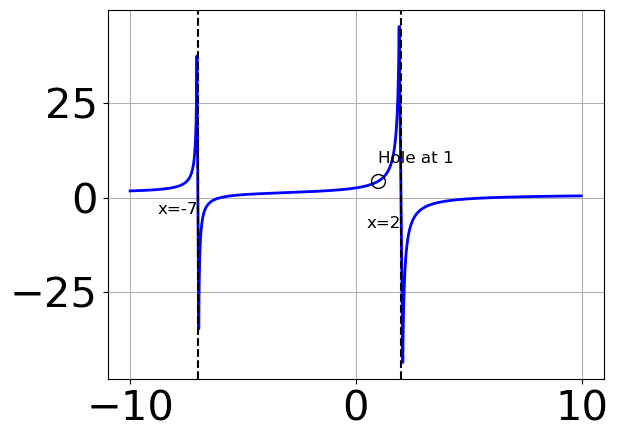
\includegraphics[width=0.5\textwidth]{../Figures/identifyGraphOfRationalFunctionCopyA.png}
\end{center}
\begin{enumerate}[label=\Alph*.]
\item \( f(x)=\frac{x^{3} + x^{2} -36.0 x -36.0}{x^{3} -4.0 x^{2} -19.0 x -14.0} \)
\item \( f(x)=\frac{x^{3} +4.0 x^{2} -36.0 x -144.0}{x^{3} -4.0 x^{2} -19.0 x -14.0} \)
\item \( f(x)=\frac{x^{3} +3.0 x^{2} -36.0 x -108.0}{x^{3} +4.0 x^{2} -19.0 x + 14.0} \)
\item \( f(x)=\frac{x^{3} -1.0 x^{2} -36.0 x + 36.0}{x^{3} +4.0 x^{2} -19.0 x + 14.0} \)
\item \( \text{None of the above are possible equations for the graph.} \)

\end{enumerate} }
\litem{
Which of the following functions \textit{could} be the graph below?
\begin{center}
    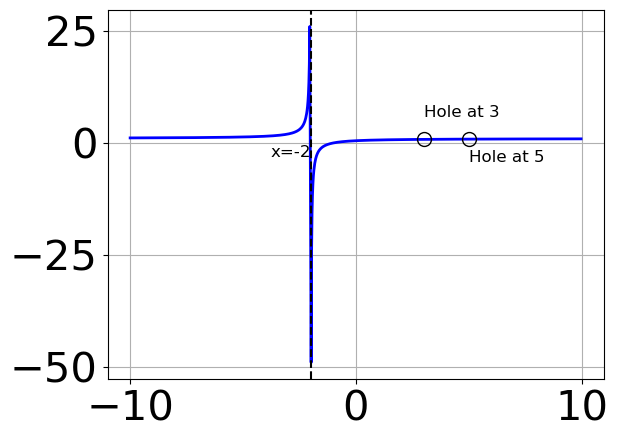
\includegraphics[width=0.5\textwidth]{../Figures/identifyGraphOfRationalFunctionA.png}
\end{center}
\begin{enumerate}[label=\Alph*.]
\item \( f(x)=\frac{x^{3} -8.0 x^{2} +13.0 x -6.0}{x^{3} +6.0 x^{2} -x -30.0} \)
\item \( f(x)=\frac{x^{3} +7.0 x^{2} +7.0 x -15.0}{x^{3} +6.0 x^{2} -x -30.0} \)
\item \( f(x)=\frac{x^{3} -31.0 x -30.0}{x^{3} -6.0 x^{2} -x + 30.0} \)
\item \( f(x)=\frac{x^{3} -7.0 x^{2} +7.0 x + 15.0}{x^{3} -6.0 x^{2} -x + 30.0} \)
\item \( \text{None of the above are possible equations for the graph.} \)

\end{enumerate} }
\litem{
Determine the vertical asymptotes and holes in the rational function below.\[ f(x) = \frac{6x^{3} -49 x^{2} +125 x -100}{9x^{2} -27 x + 20} \]\begin{enumerate}[label=\Alph*.]
\item \( \text{Holes at } x = 1.333 \text{ and } x = 1.667 \text{ with no vertical asymptotes.} \)
\item \( \text{Vertical Asymptote of } x = 0.667 \text{ and hole at } x = 1.667 \)
\item \( \text{Vertical Asymptote of } x = 1.333 \text{ and hole at } x = 1.667 \)
\item \( \text{Vertical Asymptotes of } x = 1.333 \text{ and } x = 1.667 \text{ with no holes.} \)
\item \( \text{Vertical Asymptotes of } x = 1.333 \text{ and } x = 2.5 \text{ with a hole at } x = 1.667 \)

\end{enumerate} }
\litem{
Determine the horizontal and/or oblique asymptotes in the rational function below.\[ f(x) = \frac{12x^{3} -25 x^{2} -82 x -40}{-6x^{3} -17 x^{2} +46 x + 24} \]\begin{enumerate}[label=\Alph*.]
\item \( \text{Vertical Asymptote of } y = -1.500  \)
\item \( \text{Vertical Asymptote of } y = 4  \)
\item \( \text{Horizontal Asymptote of } y = 0  \)
\item \( \text{None of the above} \)
\item \( \text{Horizontal Asymptote of } y = -2.000  \)

\end{enumerate} }
\litem{
Determine the vertical asymptotes and holes in the rational function below.\[ f(x) = \frac{6x^{3} -11 x^{2} -5 x + 12}{6x^{2} -23 x + 20} \]\begin{enumerate}[label=\Alph*.]
\item \( \text{Vertical Asymptotes of } x = 2.5 \text{ and } x = 1.333 \text{ with no holes.} \)
\item \( \text{Vertical Asymptotes of } x = 2.5 \text{ and } x = 1.5 \text{ with a hole at } x = 1.333 \)
\item \( \text{Vertical Asymptote of } x = 1.0 \text{ and hole at } x = 1.333 \)
\item \( \text{Vertical Asymptote of } x = 2.5 \text{ and hole at } x = 1.333 \)
\item \( \text{Holes at } x = 2.5 \text{ and } x = 1.333 \text{ with no vertical asymptotes.} \)

\end{enumerate} }
\litem{
Determine the horizontal and/or oblique asymptotes in the rational function below.\[ f(x) = \frac{9x^{3} +54 x^{2} +80 x + 32}{3x^{2} +8 x + 4} \]\begin{enumerate}[label=\Alph*.]
\item \( \text{Horizontal Asymptote of } y = 3.0  \)
\item \( \text{Horizontal Asymptote of } y = 3.0 \text{ and Oblique Asymptote of } y = 3x + 10 \)
\item \( \text{Horizontal Asymptote of } y = -2.0 \text{ and Oblique Asymptote of } y = 3x + 10 \)
\item \( \text{Oblique Asymptote of } y = 3x + 10. \)
\item \( \text{Horizontal Asymptote at } y = -2.0 \)

\end{enumerate} }
\litem{
Determine the horizontal and/or oblique asymptotes in the rational function below.\[ f(x) = \frac{5x^{2} +17 x -12}{10x^{3} -1 x^{2} -53 x + 30} \]\begin{enumerate}[label=\Alph*.]
\item \( \text{Horizontal Asymptote at } y = -4.000 \)
\item \( \text{Oblique Asymptote of } y = 2x -7. \)
\item \( \text{Horizontal Asymptote of } y = 0 \)
\item \( \text{Horizontal Asymptote of } y = 0.500  \)
\item \( \text{Horizontal Asymptote of } y = 0.500 \text{ and Oblique Asymptote of } y = 2x -7 \)

\end{enumerate} }
\litem{
Determine the vertical asymptotes and holes in the rational function below.\[ f(x) = \frac{8x^{3} +2 x^{2} -27 x -18}{8x^{2} -6 x -9} \]\begin{enumerate}[label=\Alph*.]
\item \( \text{Vertical Asymptote of } x = 1.5 \text{ and hole at } x = -0.75 \)
\item \( \text{Vertical Asymptotes of } x = 1.5 \text{ and } x = -1.5 \text{ with a hole at } x = -0.75 \)
\item \( \text{Vertical Asymptotes of } x = 1.5 \text{ and } x = -0.75 \text{ with no holes.} \)
\item \( \text{Vertical Asymptote of } x = 1.0 \text{ and hole at } x = -0.75 \)
\item \( \text{Holes at } x = 1.5 \text{ and } x = -0.75 \text{ with no vertical asymptotes.} \)

\end{enumerate} }
\litem{
Determine the vertical asymptotes and holes in the rational function below.\[ f(x) = \frac{8x^{3} -10 x^{2} -13 x + 15}{8x^{2} -18 x + 9} \]\begin{enumerate}[label=\Alph*.]
\item \( \text{Vertical Asymptotes of } x = 0.75 \text{ and } x = -1.25 \text{ with a hole at } x = 1.5 \)
\item \( \text{Vertical Asymptote of } x = 1.0 \text{ and hole at } x = 1.5 \)
\item \( \text{Holes at } x = 0.75 \text{ and } x = 1.5 \text{ with no vertical asymptotes.} \)
\item \( \text{Vertical Asymptotes of } x = 0.75 \text{ and } x = 1.5 \text{ with no holes.} \)
\item \( \text{Vertical Asymptote of } x = 0.75 \text{ and hole at } x = 1.5 \)

\end{enumerate} }
\end{enumerate}

\end{document}